\documentclass{article}

%math stuff
\usepackage{amsmath}
\usepackage{enumitem}
\usepackage{mathtools}
\usepackage{listings}

%bibliography/appendix
\usepackage{cite}
\usepackage[toc,page]{appendix}

%figures
\usepackage{graphicx}
\usepackage{booktabs}


%General Formating
\renewcommand*\familydefault{\sfdefault}
\usepackage{cmbright}
\usepackage[letterpaper, portrait, margin=1.5in]{geometry}
\usepackage{fancyhdr}
\pagestyle{fancy}

%Header
\lhead{Schulman}
\rhead{Page \thepage}

\title{Macro HW 9}
\author{Eric Schulman}
\date{\today}

\begin{document}


\maketitle

\section{Question 2}

\section{Question 3}

\begin{center}
    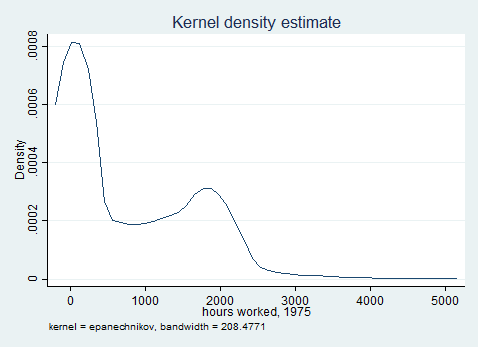
\includegraphics[scale=.6]{../plots/q3_graph}
\end{center}

\section{Question 4}

\subsection{Part (a)-(b)}

\begin{center}
    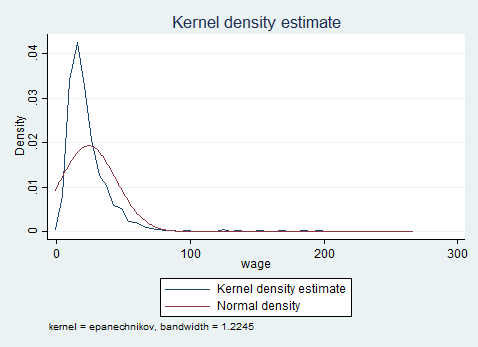
\includegraphics[scale=.6]{../plots/q4_graph1}
\end{center}

\subsection{Part (c)}

\begin{center}
    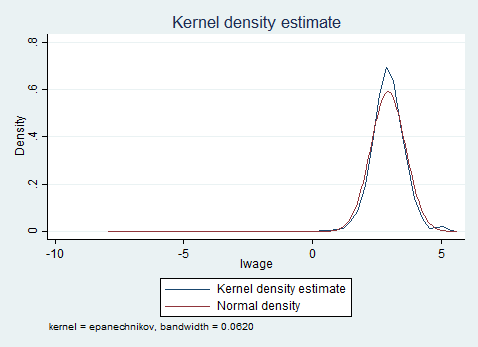
\includegraphics[scale=.6]{../plots/q4_graph2}
\end{center}

The non-parametric density function seems to capture the shape of the graph better. The data is left-skewed and slightly 'bumpy'.

\subsection{Part (d)}

\begin{center}
	\centering
    \textbf{Wage vs Experience for White Males}\par\medskip
    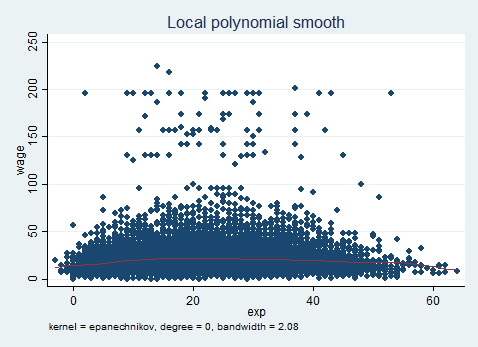
\includegraphics[scale=.6]{../plots/q4_graph3}
\end{center}

\begin{center}
	\textbf{Wage vs Experience for White Females}\par\medskip
    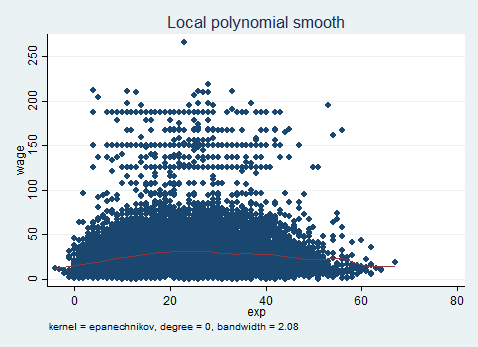
\includegraphics[scale=.6]{../plots/q4_graph4}
\end{center}

\begin{center}
	\textbf{Log(Wage) vs Experience for White Males}\par\medskip
    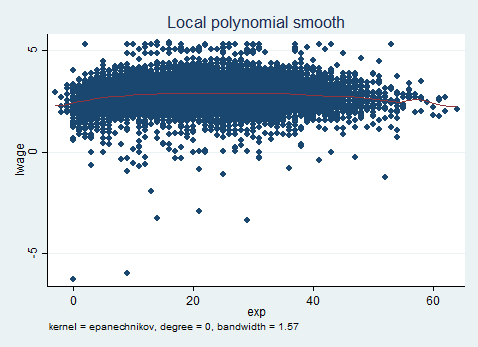
\includegraphics[scale=.6]{../plots/q4_graph5}
\end{center}

\begin{center}
\textbf{Log(Wage) vs Experience for White Females}\par\medskip
    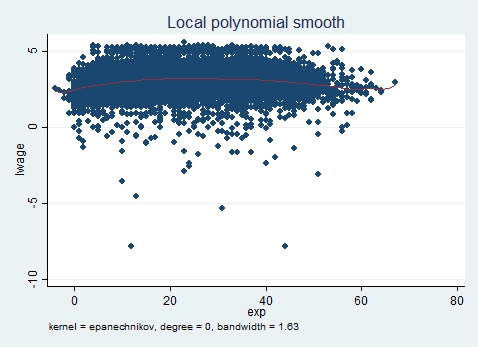
\includegraphics[scale=.6]{../plots/q4_graph6}
\end{center}

There is a lot of variation in wages that remains unexplained in the non-parametric regression. Looking at the plots, it is clear that wage experience is almost orthogonal to experience. It does have a bit of downward 'curvature' as expected.

\section{Do File}

\begin{lstlisting}
log using "C:\Users\ehs588\Downloads\hw5_output.txt", text replace

/*---------------Question 2---------------*/
use "C:\Users\ehs588\Downloads\wagepan.dta", clear
regress lwage exper expersq educ union black poorhlth
xtreg lwage exper expersq educ union black poorhlth, fe
estimates store fixed
xtreg lwage exper expersq educ union black poorhlth, re
hausman fixed ., sigmamore

/*Do it again with dummy variables*/
regress lwage exper expersq educ union black poorhlth d81 d82 d83 d84 d85 d86 d87
xtreg lwage exper expersq educ union black poorhlth d81 d82 d83 d84 d85 d86 d87, fe
estimates store fixed
xtreg lwage exper expersq educ union black poorhlth d81 d82 d83 d84 d85 d86 d87, re
hausman fixed ., sigmamore

/*---------------Question 3---------------*/

/*part (b)*/
use "C:\Users\ehs588\Downloads\MROZ.DTA", clear
mprobit inlf kidslt6 huswage kidsge6 educ
tobit hours kidslt6 huswage kidsge6 educ, ll
truncreg hours kidslt6 huswage kidsge6 educ, ll(0)

/*part (c)*/
kdensity hours
graph export "C:\Users\ehs588\Downloads\q3_graph.png", replace

/*---------------Question 4---------------*/
use "C:\Users\ehs588\Downloads\cps09mar.dta", clear

/*part (b)*/
kdensity wage, normal
graph export "C:\Users\ehs588\Downloads\q4_graph1.png", replace

/*part (c)*/
kdensity lwage, normal 
graph export "C:\Users\ehs588\Downloads\q4_graph2.png", replace

/*part d*/
lpoly wage exp if female==1 & white==1
graph export "C:\Users\ehs588\Downloads\q4_graph3.png", replace
lpoly wage exp if female==0 & white==1
graph export "C:\Users\ehs588\Downloads\q4_graph4.png", replace
lpoly lwage exp if female==1 & white==1
graph export "C:\Users\ehs588\Downloads\q4_graph5.png", replace
lpoly lwage exp if female==0 & white==1
graph export "C:\Users\ehs588\Downloads\q4_graph6.png", replace

translate "C:\Users\ehs588\Downloads\hw5_output.txt" "C:\Users\ehs588\Downloads\hw5_output.pdf"
log close

\end{lstlisting}

\end{document}
